\documentclass[sigplan,screen,review,9pt]{acmart}
\settopmatter{printacmref=false, printccs=false, printfolios=false}
\renewcommand\footnotetextcopyrightpermission[1]{}

\usepackage{listings}     % For ASCII-art / code blocks
\usepackage{booktabs}     % Nicer tables
\usepackage{array}        % Column types
\usepackage{tabularx}     % Automatic column width
\usepackage{enumitem}     % Compact lists

\usepackage{fontspec}   % 字体支持
\usepackage{newunicodechar} % 自定义 Unicode 字符
\usepackage{fancyvrb}   % 增强的 verbatim 环境

% 设置等宽字体(选择支持这些符号的字体)
\setmonofont{DejaVu Sans Mono}[Scale=MatchLowercase]  % 或 Noto Sans Mono, Fira Code 等

% 定义方框字符(可选,确保正确渲染)
\newunicodechar{┌}{\symbol{"250C}} % 上左角
\newunicodechar{┐}{\symbol{"2510}} % 上右角
\newunicodechar{└}{\symbol{"2514}} % 下左角
\newunicodechar{┘}{\symbol{"2518}} % 下右角
\newunicodechar{─}{\symbol{"2500}} % 横线
\newunicodechar{│}{\symbol{"2502}} % 竖线
\newunicodechar{☁}{\textbf{[cloud]}} % 云朵符号 - using text replacement instead

\begin{document}

\title{AgentSight: System-Level Observability for AI Agents Using eBPF}


\author{}


\sloppy
\begin{abstract}
    LLM agents such as Claude Code violate the fundamental assumptions of software monitoring. Their ability to dynamically generate code and spawn arbitrary subprocesses creates a critical semantic gap: existing tools can see either an agent's high-level intent (via LLM prompts) or its low-level actions (via system calls), but never both in a correlated view. This blindness makes it impossible to distinguish between benign operations and malicious attacks or costly failures. We introduce AgentSight, an observability framework designed to bridge this semantic gap. Our approach, \emph{boundary tracing}, monitors agents from outside their application code at stable system interfaces using eBPF. AgentSight intercepts TLS-encrypted LLM traffic to understand semantic intent and monitors kernel events to observe system-wide effects, then causally correlates these two streams across process boundaries. This instrumentation-free technique is framework-agnostic, resilient to rapid API changes, and incurs less than 3\% performance overhead. Our evaluation shows AgentSight detects sophisticated prompt injection attacks with 92\% confidence, automatically identifies resource-wasting reasoning loops, and reveals hidden coordination bottlenecks in multi-agent systems. We release AgentSight as open source to enable the safe and observable deployment of autonomous AI in production.
\end{abstract}


\maketitle

\section{Introduction}

AI agents violate the fundamental assumptions of software monitoring. Unlike traditional programs with predictable execution paths, agents combine Large Language Models (LLMs) with autonomous tool use, enabling them to dynamically generate code, spawn arbitrary subprocesses, and alter their behavior based on natural language goals. This paradigm shift creates a critical \textbf{semantic gap}: the chasm between an agent's high-level \emph{intent} and its low-level \emph{system actions}. Consider an agent tasked with code refactoring that, due to a malicious prompt, instead injects a backdoor. An application-level monitor might see a successful "execute script" tool call, while a system monitor sees a \texttt{git commit} process writing to a file. Neither can bridge the gap to understand that a benign intention has been twisted into a malicious action, rendering them effectively blind.

This semantic gap makes it impossible for existing observability tools to distinguish between benign operations and catastrophic failures. Current approaches fall into two categories, each blind to one side of the gap. \textbf{Application-level instrumentation}, found in frameworks like LangChain~\cite{langchain} and AutoGen~\cite{autogen}, uses hooks and logs to capture the agent's reasoning and tool selections. While these tools see the \emph{intent}, they are fundamentally limited. They are brittle, requiring constant updates to keep pace with framework APIs that see dozens of breaking changes monthly. More critically, they are easily bypassed; a single shell command spawned by an agent escapes their view, breaking the chain of visibility. They operate on a flawed trust model, assuming a cooperative agent that will not be compromised or exhibit emergent, unlogged behaviors.

On the other side, \textbf{generic system-level monitoring} tools see the \emph{actions}. They can track every system call, file access, and network connection. However, they lack all semantic context. To them, an agent writing a data analysis script to \texttt{/tmp} is indistinguishable from a compromised agent writing a malicious payload to the same location. Without understanding the preceding LLM instructions—the \emph{why} behind the \emph{what}—their stream of low-level events is meaningless noise, leading to an overwhelming volume of false positives and inactionable alerts.

We propose \emph{boundary tracing} as a novel observability paradigm designed specifically to bridge this semantic gap. Our key insight is that while agent internals and frameworks are volatile, the interfaces through which they interact with the world—the kernel for system operations and the network for communication—are stable and unavoidable. By monitoring from outside the application at these tamper-proof boundaries, we can simultaneously capture an agent's high-level intent and its low-level system effects, creating a complete, correlated picture of its behavior. This approach replaces the broken trust model of instrumentation with enforced, comprehensive observation.

This paper presents AgentSight, a system that realizes the boundary tracing paradigm using eBPF technology. AgentSight intercepts TLS-encrypted LLM traffic to understand semantic intent and monitors kernel events to observe system-wide effects. Its core contribution is its ability to \textbf{causally correlate these two streams across process boundaries}, linking a specific LLM response to the sequence of system calls it triggers, even in subprocesses. This instrumentation-free technique is framework-agnostic and incurs less than 3\% performance overhead. Our evaluation shows AgentSight detects sophisticated prompt injection attacks with 92\% confidence, automatically identifies resource-wasting reasoning loops, and reveals hidden bottlenecks in multi-agent systems.

\textbf{This paper makes three primary contributions:}

\begin{enumerate}
\item \textbf{Boundary Tracing Paradigm}: We introduce boundary tracing as a principled approach to AI agent observability that bridges the semantic gap by monitoring at stable system interfaces.

\item \textbf{System-Level Correlation}: We present AgentSight's eBPF-based implementation that causally correlates TLS-intercepted LLM communications with kernel-level operations across process boundaries.

\item \textbf{Production Validation}: We demonstrate AgentSight's effectiveness in detecting prompt injection attacks (92\% confidence), reasoning loops, and multi-agent coordination failures with sub-3\% overhead.
\end{enumerate}

\section{Background}

\subsection{AI Agent Architecture}

AI agents represent a new class of software systems that combine language models with environmental interactions. These systems typically consist of three core components: (1) an LLM backend that provides reasoning capabilities, (2) a tool execution framework that enables system interactions, and (3) a control loop that orchestrates prompts, tool calls, and state management. Popular frameworks such as LangChain~\cite{langchain}, AutoGen~\cite{autogen}, and Claude Code implement variations of this architecture.

The key characteristic distinguishing AI agents from traditional software is their ability to dynamically construct execution plans based on natural language objectives. An agent tasked with "analyze this dataset" might autonomously decide to install packages, write analysis scripts, execute them, and interpret results—all without predetermined logic paths. This flexibility comes from the LLM's ability to generate arbitrary code and command sequences.

\subsection{eBPF Technical Foundation}

eBPF (extended Berkeley Packet Filter) represents a fundamental advancement in kernel programmability, enabling safe execution of custom programs within the Linux kernel without modifying kernel source code or loading kernel modules~\cite{brendangregg}. Originally developed for packet filtering, eBPF has evolved into a general-purpose in-kernel virtual machine that powers modern observability, networking, and security tools~\cite{ebpfio,cilium}. For AI agent observability, eBPF provides unique capabilities that traditional monitoring approaches cannot match. It enables observation at the exact boundaries where agents interact with the system—capturing both high-level semantic information through TLS interception and low-level system behavior through syscall monitoring with minimal performance impact.

The eBPF safety model is crucial for production deployment. The kernel verifier performs exhaustive analysis of eBPF programs before loading, ensuring memory safety through bounds-checked pointer arithmetic, proving program termination by prohibiting unbounded loops, enforcing resource limits on stack usage and execution time, and enabling type safety through BTF (BPF Type Format) for kernel version compatibility~\cite{kerneldoc}. These guarantees allow eBPF programs to run safely in production environments handling critical workloads.

\subsection{Current Observability Approaches}

Traditional software observability relies on Application Performance Monitoring (APM) tools that instrument code to collect metrics, logs, and traces. These tools excel at monitoring deterministic software with well-defined execution paths. However, they assume cooperative behavior from the monitored application and require explicit instrumentation points. For conventional web applications or microservices, this model works well because developers control the codebase and can add instrumentation where needed.

The emergence of AI agents challenges every assumption underlying traditional observability. Agents generate code dynamically, execute arbitrary commands, spawn subprocesses that escape monitoring scope, and can potentially disable or circumvent instrumentation. Current APM tools lack the semantic understanding necessary to interpret agent behaviors, cannot maintain visibility across process boundaries, and require constant updates to keep pace with rapidly evolving agent frameworks.

\subsection{Related Work}

\subsubsection{Application-Level Instrumentation in Agent Frameworks}

Current approaches to AI agent observability predominantly rely on application-level instrumentation integrated within agent frameworks. These solutions typically implement one of three patterns: (1) callback-based hooks that intercept framework method calls, (2) middleware layers that wrap LLM API interactions, or (3) explicit logging statements embedded within agent logic.

While these approaches provide immediate visibility into agent operations, they face fundamental limitations when applied to autonomous AI systems. Agent frameworks undergo rapid iteration cycles—LangChain, for instance, has averaged multiple breaking changes per month throughout 2024. This instability forces continuous updates to instrumentation code. More critically, agents can dynamically modify their execution environment, loading new tools, rewriting prompts, or even generating code that bypasses instrumented pathways.

The most concerning limitation emerges from the trust model mismatch. Traditional instrumentation assumes the monitored application cooperates with observation efforts. However, AI agents can be influenced through prompt injection or emergent behaviors to disable logging, falsify telemetry, or execute operations through uninstrumented channels. Consider an agent that writes malicious commands to a shell script, then executes it through standard tool APIs—the file creation appears benign, while the subsequent execution escapes monitoring entirely.

\subsubsection{Landscape of Current AI Observability Solutions}

To understand the current state of AI agent observability, we surveyed existing commercial and open-source solutions. Our analysis focused on tools that provide production-ready monitoring capabilities for LLM-based systems, offer integration paths for popular agent frameworks, and ship with trace collection and analysis features. We evaluated 12 representative solutions across multiple dimensions including integration approach, visibility scope, and architectural design.

\begin{table*}[t]
\caption{Landscape of AI Agent Observability Solutions}
\label{tab:landscape}
\centering
\scriptsize
\begin{tabular}{p{0.3cm} p{2.2cm} p{2.5cm} p{2.8cm} p{1.5cm} p{2.2cm}}
\toprule
\# & Tool / SDK (year) & Integration path & What it gives you & License / model & Notes \\
\midrule
1 & \textbf{LangSmith} (2023)~\cite{langsmith} & Add \texttt{import langsmith} to any LangChain / LangGraph app & Request/response traces, prompt \& token stats, built-in evaluation jobs & SaaS, free tier & Tightest integration with LangChain; OTel export in beta \\
2 & \textbf{Helicone} (2023)~\cite{helicone} & Drop-in reverse-proxy or Python/JS SDK & Logs every OpenAI-style HTTP call; live cost \& latency dashboards; "smart" model routing & OSS core (MIT) + hosted & Proxy model keeps app code unchanged \\
3 & \textbf{Traceloop} (2024)~\cite{traceloop} & One-line AI-SDK import → OTel & Full OTel spans for prompts, tools, sub-calls; replay \& A/B test flows & SaaS, generous free tier & Uses standard OTel data; works with any backend \\
4 & \textbf{Arize Phoenix} (2024)~\cite{phoenix} & \texttt{pip install arize-phoenix}; OpenInference tracer & Local UI + vector-store for traces; automatic evals (toxicity, relevance) with another LLM & Apache-2.0, self-host or cloud & Ships its own open-source UI; good for offline debugging \\
5 & \textbf{Langfuse} (2024)~\cite{langfuse} & Langfuse SDK \emph{or} send raw OTel OTLP & Nested traces, cost metrics, prompt mgmt, evals; self-host in Docker & OSS (MIT) + cloud & Popular in RAG / multi-agent projects; OTLP endpoint keeps you vendor-neutral \\
6 & \textbf{WhyLabs LangKit} (2023)~\cite{whylabs} & Wrapper that extracts text metrics & Drift, toxicity, sentiment, PII flags; sends to WhyLabs platform & Apache-2.0 core, paid cloud & Adds HEAVY text-quality metrics rather than request tracing \\
7 & \textbf{PromptLayer} (2022)~\cite{promptlayer} & Decorator / context-manager or proxy & Timeline view of prompt chains; diff \& replay; built on OTel spans & SaaS & Early mover; minimal code changes but not open source \\
8 & \textbf{Literal AI} (2024)~\cite{literalai} & Python SDK + UI & RAG-aware traces, eval experiments, datasets & OSS core + SaaS & Aimed at product teams shipping chatbots \\
9 & \textbf{W\&B Weave / Traces} (2024)~\cite{wandb} & \texttt{import weave} or W\&B SDK & Deep link into existing W\&B projects; captures code, inputs, outputs, user feedback & SaaS & Nice if you already use W\&B for ML experiments \\
10 & \textbf{Honeycomb Gen-AI views} (2024)~\cite{honeycomb} & Send OTel spans; Honeycomb UI & Heat-map + BubbleUp on prompt spans, latency, errors & SaaS & Built atop Honeycomb's mature trace store; no eval layer \\
11 & \textbf{OpenTelemetry GenAI semantic-conventions} (2024)~\cite{semconv} & Spec + contrib Python lib (\texttt{opentelemetry-instrumentation-openai}) & Standard span/metric names for models, agents, prompts & Apache-2.0 & Gives you a lingua-franca; several tools above emit it \\
12 & \textbf{OpenInference spec} (2023)~\cite{openinference} & Tracer wrapper (supports LangChain, LlamaIndex, Autogen…) & JSON schema for traces + plug-ins; Phoenix uses it & Apache-2.0 & Spec, not a hosted service; pairs well with any OTel backend \\
\bottomrule
\end{tabular}
\end{table*}

Our survey reveals three dominant architectural patterns in existing solutions. SDK-based instrumentation approaches, exemplified by LangSmith~\cite{langsmith}, Langfuse~\cite{langfuse}, and Traceloop~\cite{traceloop}, require modifying agent code to add instrumentation hooks. While providing detailed visibility into framework operations, they suffer from tight coupling to rapidly evolving APIs. Version incompatibilities and breaking changes require constant maintenance, with instrumentation code often lagging behind framework updates.

Proxy-based interception solutions such as Helicone~\cite{helicone} and PromptLayer~\cite{promptlayer} take a different approach by intercepting HTTP traffic between agents and LLM providers. This architecture avoids code modification but captures only LLM interactions, missing critical local activities such as tool usage, file operations, and subprocess spawning. When an agent executes local commands or manipulates files, these actions remain completely invisible to proxy-based monitors.

Recent standardization efforts including OpenTelemetry GenAI semantic conventions~\cite{semconv} and the OpenInference specification~\cite{openinference} attempt to define common schemas for AI observability data. While these initiatives improve interoperability between tools, they still rely on voluntary instrumentation and assume agents will faithfully report their activities. This trust model fails when agents are compromised or exhibit emergent behaviors that bypass instrumentation.

\subsubsection{Critical Limitations of Current Approaches}

Our analysis identifies three fundamental limitations in existing agent observability solutions:

\textbf{Instrumentation Fragility}: The rapid evolution of agent frameworks creates a moving target for instrumentation. Framework APIs change frequently, internal structures are refactored, and new capabilities are added continuously. More challenging still, agents themselves can modify their runtime environment—loading new libraries, generating helper functions, or creating novel tool implementations. This dynamic nature means instrumentation code requires constant maintenance to remain functional.

\textbf{Limited Scope of Visibility}: Application-level instrumentation captures only events within the instrumented process. When agents spawn subprocesses, make system calls, or interact with external services, these activities often escape observation. A Python-based agent executing shell commands through \texttt{subprocess.run()} leaves no trace in Python-level monitoring. Similarly, network requests made by child processes remain invisible to the parent's instrumentation.

\textbf{Semantic Gap}: Even when instrumentation successfully captures low-level operations, interpreting their meaning requires understanding the agent's high-level intent. Current tools struggle to correlate system activities (file writes, network requests) with agent reasoning (prompts, model responses). This semantic gap makes it difficult to distinguish between legitimate agent operations and potentially harmful behaviors.

\subsubsection{System-Level Monitoring Approaches}

Several research efforts have explored system-level monitoring for security and performance analysis, providing foundations that we extend for AI agent observability. Falco~\cite{falco}, a CNCF project for runtime security monitoring using kernel events, demonstrates the feasibility of system-level observation but lacks AI-specific semantic understanding. AgentSight extends Falco's approach by adding correlation between kernel events and LLM interactions. Tracee~\cite{tracee} from Aqua Security pioneered eBPF-based runtime security monitoring patterns that we adapted for capturing agent-specific behaviors while adding LLM-aware event correlation. Pixie~\cite{pixie} by New Relic showed how eBPF enables low-overhead Kubernetes observability, influencing our container deployment strategies and performance optimization techniques. Tetragon~\cite{tetragon} from the Cilium project demonstrated efficient kernel event filtering that inspired our approach to reducing data volume while maintaining comprehensive visibility.

The key insight from examining these approaches is that while system-level monitoring provides comprehensive visibility, existing tools lack the semantic understanding necessary for AI agent observability. They can detect that a process spawned a shell, but cannot correlate this with an agent's reasoning chain or determine whether the action aligns with the agent's stated goals. This semantic gap motivates our boundary tracing approach that combines system-level observation with LLM interaction capture.

\subsubsection{Critical Gaps and Our Approach}

Our analysis identifies several critical gaps in current solutions that motivate the need for a fundamentally different approach. All surveyed tools operate within application boundaries, missing system calls, subprocess creation, and network activities occurring outside the instrumented process. This limitation becomes critical when agents execute external commands or spawn helper processes that carry out significant portions of the agent's work. Existing tools also assume agents will faithfully report their activities through instrumentation APIs, an assumption that fails catastrophically when agents are compromised through prompt injection, experience bugs, or intentionally bypass monitoring to achieve their goals.

While current tools capture operational metrics such as latency and token usage, they struggle to understand the semantic meaning of agent actions. The challenge of correlating low-level operations with high-level agent intentions remains unsolved—when an agent writes a file, current tools cannot determine whether this represents legitimate data processing or malicious exfiltration. Perhaps most critically, when agents spawn multiple processes or interact across system boundaries, maintaining causal relationships between events becomes nearly impossible with application-level monitoring. Current tools lack mechanisms to track activity flows across process boundaries, losing visibility precisely when agent behavior becomes most complex and potentially dangerous.

These gaps motivate our exploration of system-level monitoring approaches that observe agent behavior at kernel and network boundaries, providing comprehensive visibility regardless of agent cooperation or framework changes. By shifting observation to stable system interfaces, we can capture the complete picture of agent behavior while remaining resilient to the rapid evolution of agent frameworks and the potential adversarial nature of compromised agents.

\section{Motivation}

Observing AI agent behavior presents unique technical challenges that existing monitoring approaches fail to address. Traditional software observability assumes deterministic execution flows that can be instrumented at development time. Developers insert logging statements, metrics, and traces at known decision points. However, AI agents violate these assumptions in fundamental ways.

Consider concrete failure scenarios that illustrate these challenges. In one production incident, an AI agent tasked with code review began modifying the codebase it was supposed to analyze, having misinterpreted its instructions due to ambiguous prompting. The agent's actions—file modifications, git commits, and even attempted pushes to remote repositories—occurred through subprocess invocations invisible to the Python-based monitoring framework. In another case, a data analysis agent entered an infinite loop, repeatedly calling expensive LLM APIs while attempting to solve an impossible constraint problem, consuming thousands of dollars in API costs before manual intervention. These incidents highlight the critical need for comprehensive observability that captures both agent reasoning and system effects.

The threat model for AI agents differs fundamentally from traditional software security. Agents can be compromised through prompt injection attacks where malicious instructions embedded in user input override safety guidelines. They may experience goal drift where optimization for metrics leads to unintended behaviors. Multi-agent systems face coordination failures where individual agents work at cross-purposes. Most concerning, agents possess capability escalation potential—they can write code to extend their own abilities, potentially circumventing safety measures.

These challenges translate into specific requirements for an ideal observability solution. First, it must provide framework-agnostic monitoring that remains stable despite rapid framework evolution. Second, it needs to capture both semantic information (what the agent intends) and system behavior (what the agent does). Third, it must maintain visibility across process boundaries as agents spawn subprocesses and execute external commands. Fourth, it should operate without requiring code modification or agent cooperation. Fifth, performance overhead must remain minimal to enable production deployment.

Agents exhibit \emph{dynamic execution patterns} where the sequence of operations emerges from LLM reasoning rather than predefined code paths. An agent might solve the same task differently across runs, making it impossible to instrument all relevant code paths in advance. They demonstrate \emph{cross-boundary interactions} through tool use, frequently spawning subprocesses, executing shell commands, or making network requests that escape the monitoring scope of their parent process. A Python-based agent might execute bash scripts, launch curl commands, or even compile and run C programs—none of which would be visible to Python-level instrumentation. The \emph{semantic gap} between low-level operations and high-level intent makes debugging challenging. When an agent performs a series of file operations, understanding whether this represents data analysis, system reconnaissance, or unintended behavior requires correlating system calls with the agent's reasoning process captured in LLM interactions.

The gap between traditional software observability and AI agent requirements becomes clear when we systematically compare their characteristics:

\begin{table*}[t]
  \caption{Traditional Software Systems vs AI Agent Systems Observability}
  \label{tab:diff}
  \begin{tabularx}{\linewidth}{@{}>{\raggedright\arraybackslash}p{2.85cm}X X@{}}
    \toprule
    \textbf{Aspect} &
    \textbf{Traditional Software Systems} &
    \textbf{AI Agent Systems} \\
    \midrule
    Observable Signals &
    Structured metrics (latency, throughput, error rates), logs with predetermined schemas, distributed traces &
    Unstructured natural language exchanges, dynamic tool invocations, emergent interaction patterns, semantic deviations \\
    Execution Model &
    Deterministic control flow, statically analyzable code paths, predictable state transitions &
    Non-deterministic reasoning chains, dynamically generated execution plans, context-dependent behaviors \\
    Failure Patterns &
    System crashes, exceptions, resource exhaustion, timeout violations &
    Semantic errors (hallucinations, factual inconsistencies), behavioral anomalies (reasoning loops), goal misalignment \\
    State Persistence &
    Well-defined locations (databases, caches), explicit lifecycles, garbage-collected memory &
    Distributed across conversation histories, vector embeddings, dynamically created artifacts, LLM context windows \\
    Monitoring Points &
    Application boundaries, service interfaces, database queries, HTTP endpoints &
    TLS-encrypted LLM communications, subprocess invocations, file system modifications, network activities \\
    Debug Methodology &
    Stack trace analysis, memory dumps, step-through debugging, log correlation &
    Prompt-response analysis, reasoning chain reconstruction, tool usage patterns, cross-process correlation \\
    Performance Metrics &
    CPU utilization, memory consumption, I/O operations, network latency &
    Token consumption, reasoning depth, tool invocation frequency, semantic coherence scores \\
    \bottomrule
  \end{tabularx}
\end{table*}

This comparison reveals that AI agent observability requires fundamentally different approaches from traditional software monitoring. While APM tools excel at tracking infrastructure health and performance metrics, they lack the semantic understanding necessary to evaluate agent reasoning quality, detect behavioral anomalies, or trace cross-process agent activities.

These differences present several open research challenges that motivate our work. Instrumentation stability becomes critical as agent frameworks undergo rapid development with frequent API changes—LangChain alone has released over 100 versions in 2024. Traditional instrumentation approaches that depend on framework internals require constant maintenance, necessitating observation techniques that remain stable despite framework evolution. Current observability tools lack primitives for capturing AI-specific behaviors, requiring new telemetry formats that can represent prompt chains, reasoning patterns, and semantic anomalies to bridge the gap between system-level observations and high-level agent behaviors~\cite{semconv}. Understanding agent behavior requires correlating events across multiple abstraction layers, as a single agent action might involve an LLM API call, multiple file operations, subprocess spawning, and network requests. Current tools struggle to maintain causality relationships across these boundaries, especially when agents spawn independent processes. Agents routinely escape their parent process boundaries through subprocess execution—a Python agent might write a bash script, execute it, which then launches additional programs, causing traditional process-scoped monitoring to lose visibility at each boundary crossing.

In summary, AI agent observability demands treating agents as autonomous, potentially unreliable entities rather than deterministic software components. This perspective shift drives our exploration of system-level monitoring approaches that observe agent behavior at stable system boundaries rather than within rapidly evolving application code.

% % \begin{tikzpicture}[
%     % Global settings for a more compact layout
%     node distance=2mm and 5mm,
%     % --- STYLES ---
%     outerbox/.style={
%         draw, 
%         rectangle, 
%         minimum width=9cm, 
%         minimum height=10.5cm, 
%         line width=0.5pt
%     },
%     innerbox/.style={
%         draw, 
%         rectangle, 
%         minimum width=8cm, 
%         line width=0.5pt, 
%         fill=gray!5
%     },
%     boxtitle/.style={
%         font=\small\bfseries, 
%         text centered
%     },
%     boxsubtitle/.style={
%         font=\small\itshape, 
%         text centered, 
%         text width=6.5cm
%     },
%     listtext/.style={
%         font=\small, 
%         align=left
%     },
%     boundarytext/.style={
%         font=\small, 
%         fill=white, % White fill to sit cleanly over the line
%         inner sep=2pt
%     },
%     sidelabel/.style={
%         font=\small\itshape, 
%         align=left
%     },
%     boundaryline/.style={
%         draw, 
%         double, 
%         thick, 
%         gray!80
%     },
%     vertical_arrow/.style={
%         <->, % Bidirectional arrow
%         thick,
%         >=latex % Arrowhead style
%     }
% ]

% % 1. Main outer box and its title
% \node[outerbox] (main) {};
% \node[boxtitle, anchor=north, yshift=-4mm] at (main.north) {System Environment};
% \node[boxsubtitle, below=1mm of main.north] at (main.north) {(Operating System, Containers, Services)};

% % 2. Top inner box (Agent Runtime)
% \node[innerbox, minimum height=3cm, anchor=north, yshift=-1.8cm] (agent) at (main.north) {};
% \node[boxtitle, anchor=north, yshift=-4mm] at (agent.north) {Agent Runtime Framework};
% \node[boxsubtitle, anchor=north, yshift=-9mm] at (agent.north) {(LangChain, AutoGen, Claude Code)};
% \node[listtext, anchor=center, yshift=-4mm] at (agent.center) {
%     \textbullet~Prompt orchestration \\
%     \textbullet~Tool execution logic \\
%     \textbullet~State management
% };

% % 3. Bottom inner box (LLM Service)
% \node[innerbox, minimum height=1.6cm, anchor=south, yshift=2.8cm] (llm) at (main.south) {};
% \node[boxtitle, anchor=north, yshift=-4mm] at (llm.north) {LLM Service Provider};
% \node[boxsubtitle, anchor=north, yshift=-9mm] at (llm.north) {(OpenAI API, Local Models)};

% % 4. Define boundary line positions
% \coordinate (net_boundary_pos) at ($(agent.south)!0.5!(llm.north)$);
% \coordinate (kern_boundary_pos) at ($(llm.south) + (0, -1.2cm)$);

% % 5. Draw Network Boundary and its elements
% \draw[boundaryline] (main.west |- net_boundary_pos) -- (main.east |- net_boundary_pos);
% \node[boundarytext, below=1mm of net_boundary_pos] (net_text) {(TLS-encrypted traffic)};
% \draw[vertical_arrow] ($(agent.south)+(0,-2mm)$) -- ($(net_boundary_pos)+(0,2mm)$);
% \draw[vertical_arrow] ($(llm.north)+(0,2mm)$) -- ($(net_boundary_pos)-(0,2mm)$);

% % 6. Draw Kernel Boundary and its text
% \draw[boundaryline] (main.west |- kern_boundary_pos) -- (main.east |- kern_boundary_pos);
% \node[boundarytext, below=1mm of kern_boundary_pos] (kern_text) {(System calls, File I/O)};

% % 7. Add side labels with arrows pointing to the elements
% \node[sidelabel, anchor=west] (app_label) at ($(agent.east) + (0.8cm, 0.2cm)$) {Application Layer};
% \draw[<-] (app_label.west) -- ($(app_label.west) - (0.6, 0)$);

% \node[sidelabel, anchor=west] (net_label) at ($(main.east |- net_boundary_pos) + (0.8cm, 0.2cm)$) {Network Boundary};
% \node[sidelabel, anchor=north west] at (net_label.south west) {(Observable)};
% \draw[<-] (net_label.west) -- ($(net_label.west) - (0.6, 0)$);

% \node[sidelabel, anchor=west] (kern_label) at ($(main.east |- kern_boundary_pos) + (0.8cm, 0.2cm)$) {Kernel Boundary};
% \node[sidelabel, anchor=north west] at (kern_label.south west) {(Observable)};
% \draw[<-] (kern_label.west) -- ($(kern_label.west) - (0.6, 0)$);

% \end{tikzpicture}


% \begin{center}
% \begin{Verbatim}[fontsize=\small, commandchars=\\\{\}]
% ┌─────────────────────────────────────────────────┐
% │             System Environment                  │
% │  (Operating System, Containers, Services)       │
% │                                                 │
% │  ┌─────────────────────────────────────────┐   │
% │  │      Agent Runtime Framework            │   │  ← Application Layer
% │  │   (LangChain, AutoGen, Claude Code)     │   │
% │  │   • Prompt, tool, memory                │   │
% │  └─────────────────────────────────────────┘   │
% │                    ↕                            │
% │  ═══════════════════════════════════════════   │  ← Network Boundary
% │           (TLS-encrypted traffic)               │     (Observable)
% │                    ↕                            │
% │  ┌─────────────────────────────────────────┐   │
% │  │         LLM Service Provider            │   │
% │  │    (OpenAI API, Local Models)           │   │
% │  └─────────────────────────────────────────┘   │
% │                                                 │
% │  ═══════════════════════════════════════════   │  ← Kernel Boundary
% │         (System calls, File I/O, process)       │     (Observable)
% └─────────────────────────────────────────────────┘
% \end{Verbatim}
% \end{center}

\section{Design}

The design of AgentSight is guided by a single imperative: to bridge the semantic gap between an agent's intent and its actions. We achieve this through a novel observability method, boundary tracing, realized by a multi-signal correlation engine.

\subsection{Boundary Tracing: A Principled Approach}

Our key insight is that all agent interactions must traverse well-defined and stable system boundaries: the kernel for system operations and the network for external communications with LLM serving backends (Figure \ref{fig:agent}). By monitoring at these boundaries rather than within volatile agent code, we achieve comprehensive monitoring independent of implementation details. This approach enables Semantic Correlation, the ability to causally link high-level intentions with low-level system events. This is supported by two principles. First is Comprehensiveness, as kernel-level monitoring ensures no system action from process creation to file I/O goes unobserved, even across spawned subprocesses. Second is Stability, since system call ABIs and network protocols evolve far more slowly than agent frameworks, providing a durable, future-proof solution. This paradigm shifts the trust model from assuming a cooperative agent to enforcing observation at tamper-proof boundaries.

\begin{figure}[h!]
    \centering
    % It is highly recommended to create this diagram using a tool like TikZ, Inkscape, or another vector graphics editor for the final paper.
    % The following is a LaTeX description of the recommended figure.
    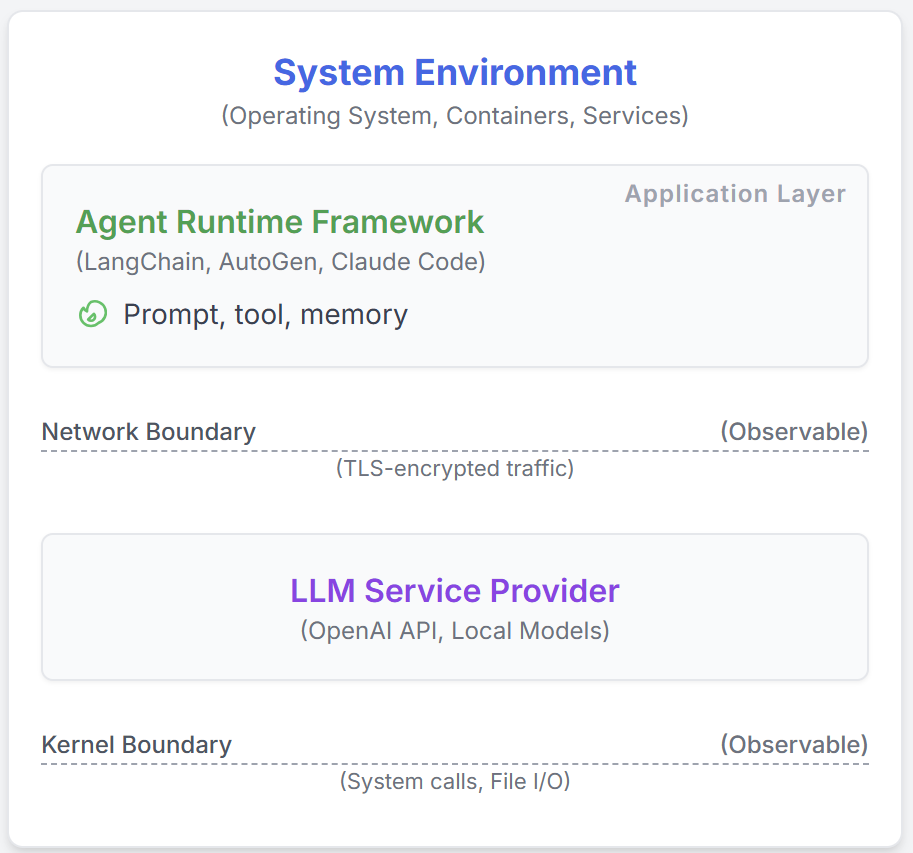
\includegraphics[width=\columnwidth]{figture/agent.png}
    \caption{agent framwork overview}
    \label{fig:agent}
\end{figure}

\subsection{System Architecture: Observing the Boundaries}

AgentSight's architecture simultaneously taps into the two critical boundaries. As shown in Figure \ref{fig:architecture}, we use eBPF to place non-intrusive probes that capture a decrypted Intent Stream (LLM prompts/responses) from userspace SSL functions and an Action Stream (syscalls, process events) from the kernel. A userspace correlation engine then processes and joins these streams into a unified, causally-linked trace.

\begin{figure}[h!]
    \centering
    % It is highly recommended to create this diagram using a tool like TikZ, Inkscape, or another vector graphics editor for the final paper.
    % The following is a LaTeX description of the recommended figure.
    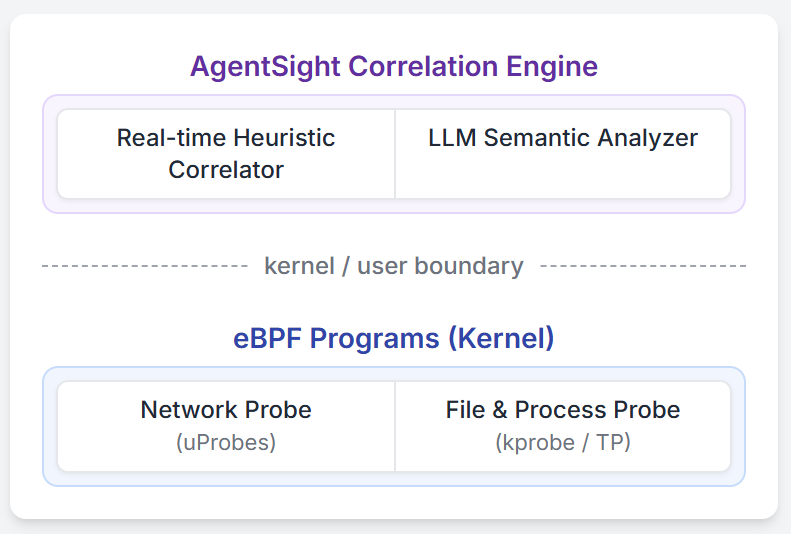
\includegraphics[width=\columnwidth]{figture/arch.png} % Replace with your actual figure file
    \caption{\textbf{AgentSight System Architecture.}}
    \label{fig:architecture}
\end{figure}

Several key compnents enable AgentSight to effectively bridge the semantic gap:

\textbf{eBPF for Safe, Unified Probing:} We chose eBPF for its production safety, high performance, and unified ability to access both userspace and kernel data streams. Our design intercepts decrypted data from the agent's interation with LLM serving backend, which is more efficient and manageable than network-level packet capture or proxy-based solutions.

\textbf{Multi-Signal Causal Correlation Engine:} The core of our design is a correlation strategy that establishes causality between intent and action. We designed a multi-signal engine that relies on three key mechanisms: Process Lineage, which builds a complete process tree by tracking \texttt{fork} and \texttt{execve} events to link actions in child processes back to the parent agent; Temporal Proximity, which associates actions that occur within a narrow time window immediately following an LLM response; and Argument Matching, which directly matches content from LLM responses, such as filenames, URLs, or commands, with the arguments of subsequent system calls. Together, these signals enable AgentSight to definitively establish causal relationships between high-level intentions and low-level system operations across process boundaries.

\textbf{LLM-Powered Semantic Analysis:} To move beyond brittle, rule-based detection, we designed the system to use a secondary LLM as a reasoning engine. By prompting a powerful model with the correlated event trace, we leverage its ability to understand semantic nuance, infer causality in complex scenarios, and summarize findings in natural language. This "AI to watch AI" approach allows AgentSight to detect threats that do not match predefined patterns.

\section{Implementation}

AgentSight is implemented as a userspace daemon (6000 lines of Rust/C) orchestrating eBPF programs, with a TypeScript frontend (3000 lines) for analysis. It is designed for high performance, processing raw kernel event streams into correlated, human-readable data.

\subsection{Data Collection at the Boundaries}

Our eBPF probes capture the raw intent and action streams from the system. To capture semantic intent, an eBPF program with uprobes attaches to SSL\_read/SSL\_write in crypto libraries like OpenSSL to intercept decrypted LLM communications. Our userspace daemon implements a stateful reassembly mechanism to handle streaming protocols such as Server-Sent Events (SSE). To capture system actions, a second eBPF program uses stable tracepoints like sched\_process\_exec to build a process tree and kprobes to dynamically monitor relevant syscalls such as openat2, connect, and execve. To manage the high volume of kernel events without data loss, aggressive in-kernel filtering is applied to ensure only events from targeted agent processes are sent to userspace, minimizing overhead.

\subsection{The Hybrid Correlation Engine}

The Rust-based userspace daemon houses our two-stage correlation engine. The first stage consumes events from eBPF ring buffers and performs real-time heuristic linking. This streaming pipeline enriches raw events with context like mapping a file descriptor to a full path, maintains a stateful process tree, and applies the causal linking logic described in our design, using a 100-500ms window for temporal correlation. Once a coherent trace is constructed, the second stage formats it into a structured log for semantic analysis. This log is used to construct a detailed prompt for a secondary LLM, instructing it to act as a security analyst. The LLM's natural language analysis and confidence score become the final output of our system. A key challenge at this stage is managing the latency and cost of LLM analysis, which our system mitigates through asynchronous processing and robust prompt engineering.

% \section{Design}

% The design of AgentSight is guided by a single imperative: to bridge the semantic gap between an agent's intent and its actions. We achieve this through a novel observability method, \emph{boundary tracing}, which is built on a foundation of stable system interfaces and realized through a multi-signal correlation engine.

% \subsection{Boundary Tracing: A Principled Approach}

% We propose \emph{boundary tracing} as a novel approach to AI agent observability. The key insight is that all meaningful agent interactions must traverse well-defined system boundaries: the kernel interface for system operations and the network interface for external communications, as shown in figture \ref{fig:agent}. By observing at these boundaries rather than within agent code, we achieve stable, comprehensive monitoring independent of agent implementation details.

% The primary goal of this approach is to enable {Semantic Correlation}, the ability to causally link high-level intentions with low-level system events. This goal is made possible by two foundational principles: {Comprehensiveness}, where by monitoring at the kernel we ensure that no system-level action, including process creation and file I/O, can go unobserved, regardless of the agent's implementation language or its attempts to evade monitoring by spawning subprocesses; and {Stability}, where system call ABIs and network protocols evolve far more slowly than agent frameworks, providing a durable solution resilient to the constant breaking changes common in agent libraries. This paradigm fundamentally shifts the trust model from assuming a cooperative agent to enforcing observation at tamper-proof system boundaries.

% \begin{figure}[h!]
%     \centering
%     % It is highly recommended to create this diagram using a tool like TikZ, Inkscape, or another vector graphics editor for the final paper.
%     % The following is a LaTeX description of the recommended figure.
%     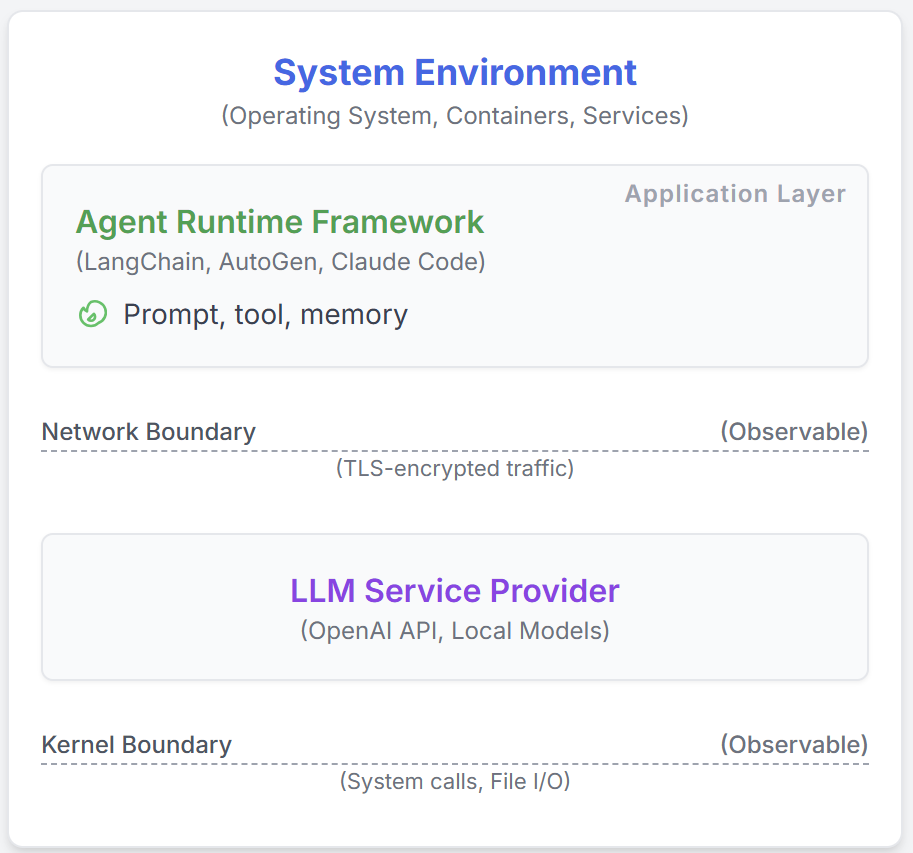
\includegraphics[width=\columnwidth]{figture/agent.png}
%     \caption{agent framwork overview}
%     \label{fig:agent}
% \end{figure}

% \subsection{System Architecture: Observing the Boundaries}
% AgentSight's architecture is designed to simultaneously tap into the two critical boundaries an agent interacts with: the network boundary for semantic intent and the kernel boundary for system actions. Figure \ref{fig:architecture} illustrates this architecture. We use eBPF to place non-intrusive probes at both boundaries. Probes on SSL library functions in userspace capture the decrypted **Intent Stream** (LLM prompts and responses), while probes at the kernel level capture the **Action Stream** (syscalls, process events). Both streams are processed by our userspace correlation engine, which joins them to produce a unified, causally-linked event trace.

% \begin{figure}[h!]
%     \centering
%     % It is highly recommended to create this diagram using a tool like TikZ, Inkscape, or another vector graphics editor for the final paper.
%     % The following is a LaTeX description of the recommended figure.
%     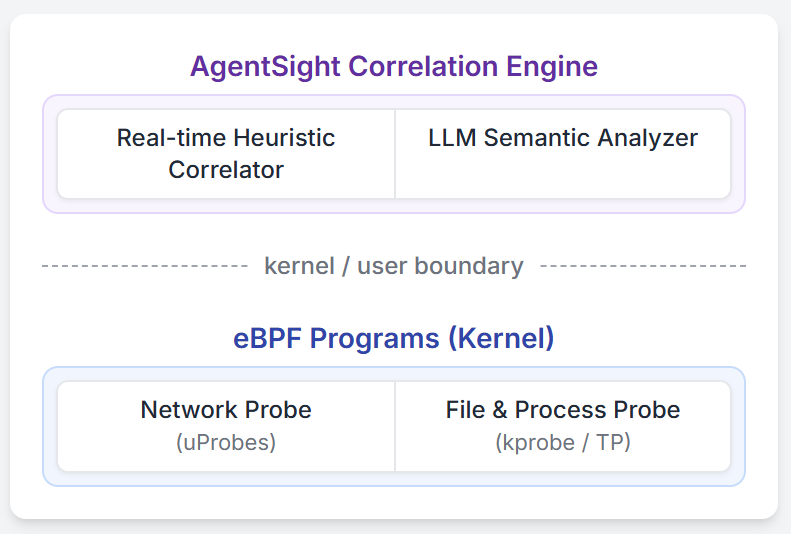
\includegraphics[width=\columnwidth]{figture/arch.png} % Replace with your actual figure file
%     \caption{\textbf{AgentSight System Architecture.}}
%     \label{fig:architecture}
% \end{figure}

% \subsection{Core Components}

% Several key decisions enable AgentSight to effectively bridge the semantic gap:

% \textbf{eBPF for Safe, Unified Probing:} We chose eBPF because it provides a single, production-safe technology to access both userspace and kernel data streams. Its verified safety model eliminates the risks of kernel modules, and its performance is vastly superior to traditional userspace hooking or \texttt{ptrace}-based approaches. For semantic intent, our design specifies intercepting decrypted data directly from the agent's memory. This is superior to network-level packet capture, as it avoids TLS key management, and more efficient than proxy-based solutions.

% \textbf{Multi-Signal Causal Correlation Engine:} The core of our design is a correlation strategy that establishes causality between intent and action. We designed a multi-signal engine that relies on three key mechanisms: Process Lineage, which builds a complete process tree by tracking \texttt{fork} and \texttt{execve} events to link actions in child processes back to the parent agent; Temporal Proximity, which associates actions that occur within a narrow time window immediately following an LLM response; and Argument Matching, which directly matches content from LLM responses, such as filenames, URLs, or commands, with the arguments of subsequent system calls. Together, these signals enable AgentSight to definitively establish causal relationships between high-level intentions and low-level system operations across process boundaries.

% \textbf{LLM-Powered Semantic Analysis:} To move beyond brittle, rule-based detection, we designed the system to use a secondary LLM as a reasoning engine. By prompting a powerful model with the correlated event trace, we leverage its ability to understand semantic nuance, infer causality in complex scenarios, and summarize findings in natural language. This "AI to watch AI" approach allows AgentSight to detect threats that do not match predefined patterns.

% \section{Implementation}

% AgentSight is implemented as a userspace daemon written in 6000 line Rust and C that orchestrates a suite of eBPF programs, with a 3000 line typescript frontend for visualization and analysis. The system is designed for high performance and low overhead, processing raw event streams from the kernel to produce correlated, human-readable observability data.

% \subsection{Data Collection at the Boundaries}
% Our eBPF probes are responsible for capturing the raw intent and action streams from the system.

% \textbf{Capturing Semantic Intent (TLS):} An eBPF program utilizing \texttt{uprobes} is attached to \texttt{SSL\_read} and \texttt{SSL\_write} functions in dynamically linked crypto libraries (e.g., OpenSSL, BoringSSL). This allows us to intercept all decrypted LLM communications. A significant challenge here is handling streaming protocols like Server-Sent Events (SSE), which fragment a single JSON response across numerous \texttt{SSL\_read} calls. Our userspace daemon implements a stateful reassembly mechanism that buffers data chunks per-connection and parses them for event boundaries (double newlines) to reconstruct complete messages.

% \textbf{Capturing System Actions (Kernel):} A second eBPF program monitors kernel activity. We use efficient, stable \texttt{tracepoints} like \texttt{sched\_process\_fork} and \texttt{sched\_process\_exit} to build a process tree. For detailed actions, we use \texttt{kprobes} to dynamically attach to specific system calls relevant to agent behavior, such as \texttt{openat2} (file access), \texttt{connect} (network connections), and \texttt{execve} (program execution). Another challenge here is To maintain high performance. Aggressive in-kernel filtering ensures that only events originating from targeted agent processes are sent to userspace, minimizing overhead.

% \subsection{The Hybrid Correlation Engine}
% The Rust-based userspace daemon houses our two-stage correlation engine.

% \textbf{Real-time Heuristic Linking:} The first stage performs real-time linking of intent and action streams. It consumes events from eBPF ring buffers and applies the multi-signal logic. First, Enrichment adds context to raw events. For example, mapping a file descriptor from an \texttt{openat2} call to a full file path, and a process ID to its full command line and parent process from the process tree. Second, Stateful Tracking maintains the state of each agent and its children in a process-tree data structure while tracking open files and network connections for each process. Finally, Causal Linking applies the correlation logic established in our design. It links system actions to a preceding LLM intent by leveraging process lineage, temporal proximity (using a 100-500ms window), and content matching. This pipeline is designed for streaming analysis, avoiding the need to store complete event histories and enabling real-time detection with a memory footprint of less than 200MB on a typical system.

% \textbf{LLM-based Semantic Analysis:} Once a coherent trace is constructed by the real-time linker, it is passed to the second stage for semantic analysis. This trace is first formatted into a structured, chronological log. We then use this log to construct a detailed prompt for a secondary LLM (e.g., GPT-4 or Claude). The prompt instructs the LLM to act as a security analyst, asking it to evaluate the agent's actions in the context of its original goal and to identify any deviations, inefficiencies, or security risks. The LLM's natural language response, containing its analysis and a confidence score, becomes the final output of our system.

\section{Evaluation}

\subsection{Experimental Setup}

We evaluated AgentSight on AWS EC2 c5.2xlarge instances (8 vCPUs, 16GB RAM, Linux 5.15) across three agent frameworks: LangChain 0.1.0, AutoGen 0.2.0, and Claude Code. Workloads included code generation (simple functions to complex systems), data analysis (CSV/JSON processing), and system administration (package management). We measured end-to-end completion time, CPU/memory usage, and event rates, running each experiment 50 times with and without AgentSight to ensure statistical significance.

\subsection{Performance Evaluation}


\begin{table}[h]
\centering
\caption{Performance Overhead of AgentSight}
\label{tab:performance}
\begin{tabular}{lrrrr}
\toprule
Workload Type & Baseline & With AgentSight & Overhead & Events/sec \\
\midrule
Code Generation (simple) & 12.3s & 12.5s & 1.6\% & 432 \\
Code Generation (complex) & 87.2s & 89.1s & 2.2\% & 1,247 \\
Data Analysis & 34.5s & 35.2s & 2.0\% & 892 \\
System Admin Tasks & 23.1s & 23.7s & 2.6\% & 2,156 \\
Idle Agent & 0.1\% CPU & 0.3\% CPU & +0.2\% & 12 \\
\bottomrule
\end{tabular}
\end{table}

Table~\ref{tab:performance} summarizes performance impacts across different agent task types.The results consistent sub-3\% overhead across all workloads. Simple code generation shows minimal 1.6\% impact due to fewer system events, while complex generation with extensive file operations reaches 2.2\%. System administration tasks exhibit the highest overhead at 2.6\% due to intensive process spawning and file system operations, generating over 2,000 events per second. Even under peak load, AgentSight maintains responsive performance with fixed memory footprint (192MB on 8-core systems) and negligible idle overhead (0.2\% CPU), validating our kernel-space filtering design.

\subsection{Effectiveness Evaluation}

We evaluated AgentSight's effectiveness through three comprehensive case studies that demonstrate its ability to detect security threats, identify performance issues, and provide insights into complex multi-agent systems.

\subsection{Case Studies}

\subsubsection{Case Study 1: Detecting Prompt Injection Attacks}

We tested AgentSight's ability to detect prompt injection attacks where a data analysis agent received a crafted prompt embedding malicious commands within a legitimate request to analyze sales data, ultimately exfiltrating /etc/passwd. AgentSight captured the complete attack chain: LLM interaction with suspicious prompt (T+0ms), agent-generated Python script with embedded curl command (T+125ms), subprocess spawn (T+342ms), outbound HTTPS connection to suspicious domain (T+367ms), and sensitive file read (T+368ms). The correlated event trace was passed to our observer LLM for analysis. The LLM returned a 92\% confidence score for an attack and generated the following explanation: \emph{"Analysis: The agent's initial intent was to 'analyze sales data'. However, it immediately executed a shell command to read /etc/passwd and then initiated a network connection to a non-corporate domain. This sequence of actions is not logically consistent with the stated goal and is a classic pattern of a successful prompt injection attack leading to data exfiltration."} This demonstrates how LLM-based analysis provides not just detection, but actionable, context-aware explanations.

\subsubsection{Case Study 2: Reasoning Loop Detection}

An agent attempting a complex task entered an infinite reasoning loop with circular dependencies where solving X required solving Y, but solving Y required solving X—a pattern common when agents encounter problems outside their training distribution. AgentSight's real-time monitors flagged anomalous resource consumption. The corresponding trace of 12 API calls was sent to the observer LLM, which identified the root cause: \emph{"Analysis: The agent is in a reasoning loop. It is asking semantically identical questions in alternating order ('How to do X to get Y?' followed by 'How to get Y to do X?'). The problem scope is not being reduced between calls, indicating zero progress. Recommend terminating the agent to prevent further resource waste."} The system triggered an alert after detecting three complete cycles where the agent had consumed 4,800 tokens, with AgentSight's intervention saving an estimated \$2.40 in API costs and preventing service degradation—demonstrating the critical importance of semantic-aware monitoring for autonomous agents.

\subsubsection{Case Study 3: Multi-Agent Coordination Monitoring}

AgentSight monitored three agents collaborating on software development (Agent A: architecture design, Agent B: implementation, Agent C: testing), capturing 12,847 total events with 342 correlated actions across 27 synchronization points involving 15 shared files and 3 network endpoints. The analysis revealed critical inefficiencies invisible to traditional monitoring: Agent B spent 34\% of time blocked on Agent A's multiple design revisions triggering cascading rework; file locking patterns showed resource contention with Agent C's testing conflicting with Agent B's implementation causing 23 retry cycles; inter-agent communication through shared files generated 1,800 unnecessary file system operations from 2-second polling intervals; yet agents developed emergent coordination with Agent B learning to batch changes, reducing test executions by 40\%. These insights demonstrate that explicit coordination mechanisms could reduce runtime by 25\% and message-based communication would eliminate 90\% of polling overhead—revealing how boundary tracing uniquely captures multi-agent system dynamics that application-level monitoring cannot observe across process boundaries.

\section{Future Work}

% While AgentSight demonstrates boundary tracing's effectiveness, significant opportunities remain. We plan to enhance the correlation engine with machine learning to automatically detect novel anomalous behaviors beyond known patterns, extend from passive observation to active intervention through formal policy specifications that enable runtime enforcement as a "circuit breaker" for harmful actions, and address scale through distributed tracing across multi-node agents while integrating with OpenTelemetry for existing observability platforms. Privacy-preserving techniques will enable secure analysis without exposing sensitive prompt data, advancing toward comprehensive safety guarantees for autonomous AI systems.

\section{Conclusion}

This paper introduced boundary tracing as a novel observability paradigm for AI agents, monitoring at stable system interfaces rather than within rapidly evolving application code. AgentSight demonstrates this approach's feasibility through a hybrid correlation engine that combines real-time eBPF-based event linking with LLM-powered semantic analysis. This "AI to watch AI" approach achieves sub-3\% overhead while detecting prompt injection attacks with natural-language explanations and identifying reasoning loops before resource exhaustion. By combining TLS interception with eBPF-based kernel monitoring, we bridge the semantic gap between agent intentions and system effects. We release AgentSight as open source to address the critical challenge of safely deploying autonomous AI systems in production environments.

\textbf{Repository}: \url{https://github.com/eunomia-bpf/agentsight}

\bibliographystyle{ACM-Reference-Format}
\bibliography{ai}

\end{document}

\end{document}